\section{Polarization of Light}
This section is based on Section 1.7 of University Physics Volume 3 \cite[30-33]{lingUniversityPhysicsVolume2016}.
Light is an electromagnetic (EM) wave with oscillating electric and magnetic fields perpendicular to its direction of propagation.
The specific orientation of these oscillations is referred to as polarization.
Natural light sources, such as the Sun, emit unpolarized light in which the electric fields have random orientations, encompassing various polarization directions.

Polarizing filters can transmit light waves with polarization aligned with the filter's orientation while blocking waves that are not aligned.
This behavior follows Malus's law, which describes the relationship between the intensity of polarized light transmitted through a polarizer and the angle between the polarization direction of the incident light and the orientation of the polarizer:
\begin{equation}
    I = I_0 cos^2 \theta
\end{equation}

\subsection{Polarization Properties of Reflected Light}
Unpolarized light becomes partially polarized when reflected off a surface \cite[34]{lingUniversityPhysicsVolume2016}.
This is the reason why sunglasses are commonly polarized, as they are designed to block reflected light from surfaces such as roads or water.
Figure \ref{fig:polarized_reflection} illustrates this phenomenon where the light gets partially polarized parallel to the surface (perpendicular to the plane of incidence).
At one particular angle of incidence, the reflected light is completely polarized parallel to the surface.
This angle is called the Brewster angle and is given by \cite{BrewsterAngle2023}:

\begin{equation}
    \theta_B = \arctan{\frac{n_2}{n_1}}
\end{equation}

\begin{figure}[H]
    \centering
    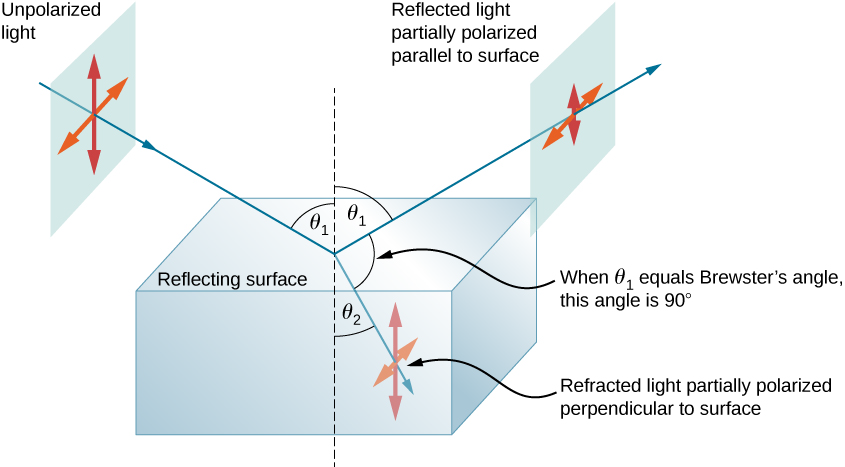
\includegraphics[width=\textwidth]{figures/polarization/reflaction.png}
    \caption{Polarization by reflection. \cite[Figure 1.38]{lingUniversityPhysicsVolume2016}}
    \label{fig:polarized_reflection}
\end{figure}


Any polarization state can be resolved as a sum of two orthogonal linear polarizations where one is perpendicular to the plane of incidence $R_\perp$ and the other is parallel to the plane of incidence $R_\parallel$ \cite{FresnelEquations2023}.
These two components are referred to as s-polarized and p-polarized light, respectively and their reflection coefficients are given by the Fresnel equations \cite{FresnelEquations2023}:

\begin{align}
    \centering
    R_\perp =         & \left|{\frac {n_{1}\cos \theta _1-n_{2}\cos \theta _2}{n_{1}\cos \theta _1+n_{2}\cos \theta _2}}\right|^{2} \\
    \\
    R_\parallel     = & \left|{\frac {n_{1}\cos \theta _2-n_{2}\cos \theta _1}{n_{1}\cos \theta _2+n_{2}\cos \theta _1}}\right|^{2}
\end{align}

Where  $\eta_1$ and $\eta_2$ are the refractive indices of the two media,
$\theta_i$ is the angle of incidence and $\theta_r$ is the angle of refraction.

Using the trigonometric identity $ \cos^2{\left(\theta_2 \right)} = 1- \sin^2{\left(\theta_2 \right)}$ and Snell's law $\eta_1 \sin{\left(\theta_1 \right)} = \eta_2 \sin{\left(\theta_2 \right)}$ the angle of refraction, $\theta_2$ can be removed, and the equations can be written as:

\begin{align}
    R_\perp =         & \left|{\frac {n_{1}\cos \theta _1-n_{2}{\sqrt {1-\left({\frac {n_{1}}{n_{2}}}\sin \theta _1\right)^{2}}}}{n_{1}\cos \theta _1+n_{2}{\sqrt {1-\left({\frac {n_{1}}{n_{2}}}\sin \theta _1\right)^{2}}}}}\right|^{2} \\
    \\
    R_\parallel     = & \left|{\frac {n_{1}{\sqrt {1-\left({\frac {n_{1}}{n_{2}}}\sin \theta _1\right)^{2}}}-n_{2}\cos \theta _1}{n_{1}{\sqrt {1-\left({\frac {n_{1}}{n_{2}}}\sin \theta _1\right)^{2}}}+n_{2}\cos \theta _1}}\right|^{2}
\end{align}


Inserting the refractive index of air, $n_1 = 1$, and the refractive index of water, $n_2 = 1.33$, the reflectance can be calculated and plotted as a function of the angle of incidence, $\theta_1$, alone as shown in Figure \ref{fig:brewster0}.


\begin{figure}[H]
    \centering
    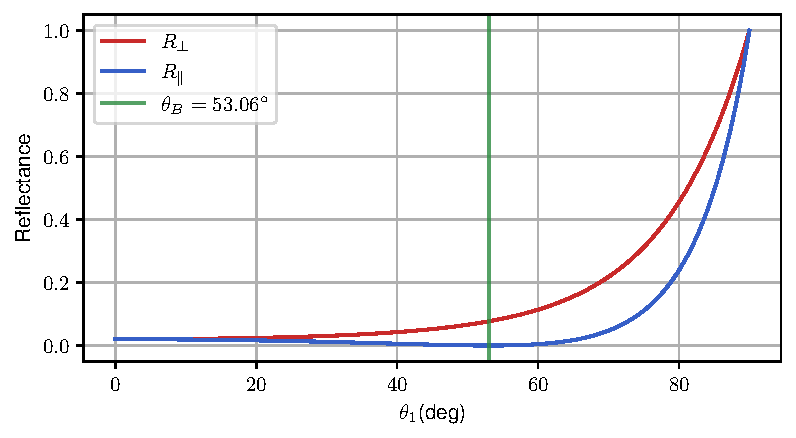
\includegraphics[width=\textwidth]{figures/pol_plots/brewster0.pdf}
    \caption{Reflectance of S and P polarized light of water as a function of the angle of incidence.}
    \label{fig:brewster0}
\end{figure}

The \gls{dolp} is the degree to which light is polarized and can be defined as the ratio between the difference and the sum of the two components:

\begin{align}
    DoLP= & \frac{\left | R_\perp - R_\parallel \right |}{R_\perp + R_\parallel}
\end{align}
\begin{figure}[H]
    \centering
    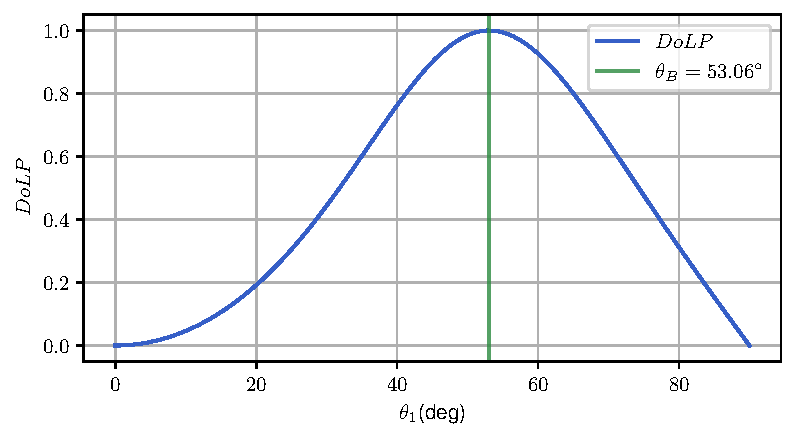
\includegraphics[width=\textwidth]{figures/pol_plots/brewster1.pdf}
    \caption{\gls{dolp} of light reflected off water as a function of the angle of incidence.}
    \label{fig:brewster1}
\end{figure}

